\section{Experiments and Results}
\label{sec:experiments}

\subsection{Experimental setup}
The primary task is PyBullet pick-and-place with a Franka Panda. The 10D state
contains end-effector, cube, and goal positions (three coordinates each) plus
mean finger opening. The action is a 3D Cartesian delta and binary gripper
command. Target radius affects success and Task difficulty but is not observed
by the policy.
A deterministic finite-state expert physically grasps, transports, releases,
and retreats. We collect 300 successful demonstrations (65,738 transitions)
and freeze a trajectory-level 240/60 train/validation split. Policies use a
$10\!\rightarrow\!128\!\rightarrow\!128$ ReLU MLP with separate motion and
gripper heads. AdamW uses learning rate $10^{-3}$ and batch size 256. Each
curriculum has 20,600 updates and seeds 5478, 5479, and 5480. Evaluation tasks
and difficulty groups are frozen before policy comparison. An episode succeeds
when cube--goal horizontal distance is below the sampled radius and vertical
error is below 0.025~m; the horizon is 400 actions.

The demonstrations are generated by a closed-loop finite-state controller,
not by teleporting the cube or constraining it to the gripper. Each trajectory
includes physical approach, finger closure, lift, transport, placement,
release, and retreat. Cube and goal $x$ positions vary in $[0.42,0.63]$~m;
their $y$ ranges are $[-0.28,0.12]$ and $[-0.12,0.28]$~m, with at least
0.18~m separation. Target radii vary in $[0.045,0.075]$~m, while robot
initialization and simulator settings remain fixed. Dataset and
evaluation-task fingerprints prevent accidental regeneration or overlap.
Complete trajectories, rather than individual transitions, are assigned to
training and validation sets.

Figure~\ref{fig:pnp-simulation-sequence} shows one deterministic successful
expert rollout rendered directly by the PyBullet camera. The four frames come
from the same trajectory and show the physical finger grasp, lifted transport,
and release over the goal marker.

\begin{figure*}[t]
  \centering
  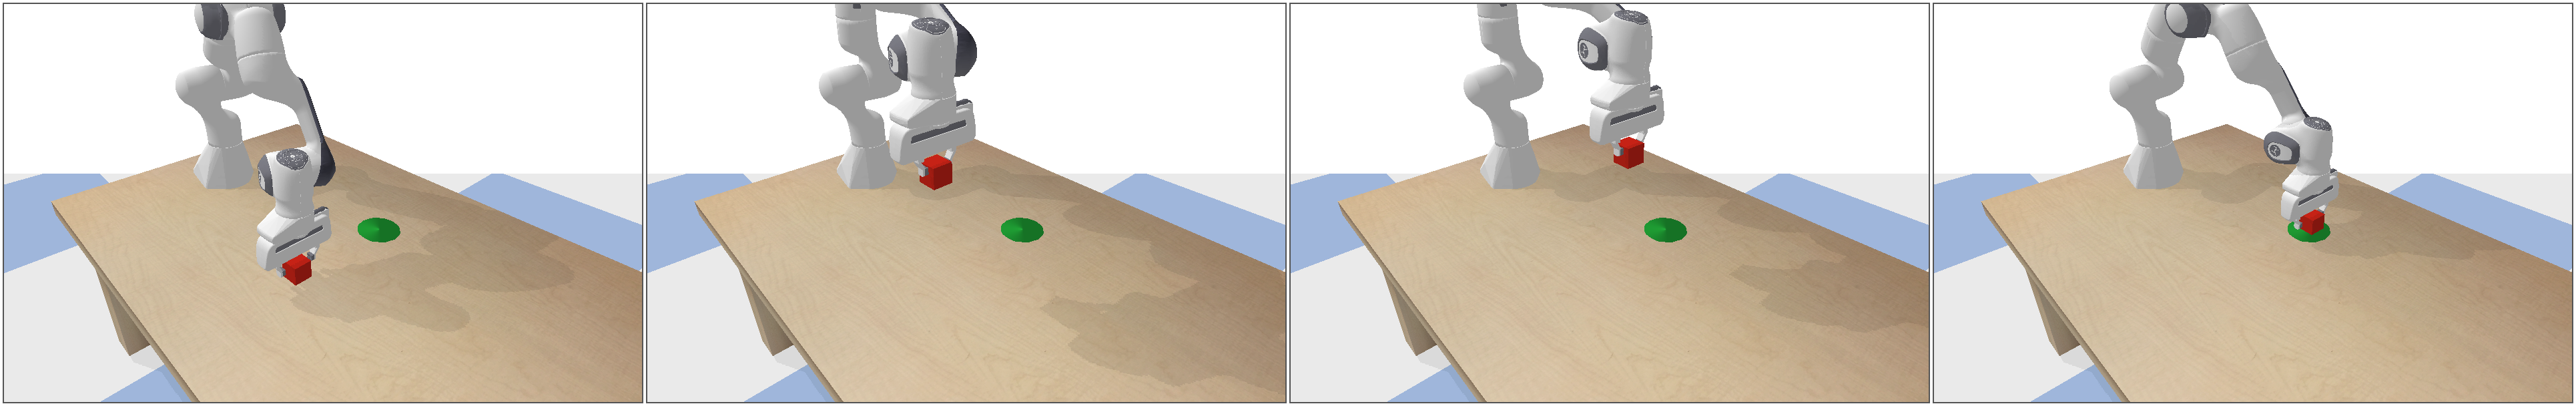
\includegraphics[width=\textwidth]{figures/pnp_simulation_sequence.png}
  \caption{Real PyBullet states from one successful deterministic
  pick-and-place expert rollout: (a) final pre-grasp approach, (b) grasped
  cube after lift, (c) mid-transport, and (d) placement and gripper release.
  The robot advances only through the environment action interface; the cube
  is neither teleported nor attached by an artificial constraint.}
  \label{fig:pnp-simulation-sequence}
\end{figure*}

An initial unscaled policy reaches 0/100 closed-loop success despite high
offline gripper accuracy. Scaling Cartesian targets by the maximum expert step
($0.008$~m) reduces validation motion error and raises a separately developed
Uniform baseline to 83/100. All controlled curriculum runs use this scaled
formulation from scratch; the historical 83/100 checkpoint is not substituted
for matched Uniform. This prevents a development-selected checkpoint from
receiving an unfair advantage in the controlled comparison.

The 60-trajectory validation split supplies offline loss only. Closed-loop
learning curves use a separate frozen 100-task development set. Final reporting
uses 200 new Fresh-ID tasks and two disjoint 100-task OOD sets; none selects a
checkpoint.

\subsection{Difficulty metrics and failure prediction}
\label{sec:difficulty-results}
The metrics disagree substantially (Figure~\ref{fig:pnp-corr}). Spearman
correlations are $0.842$ (Task--Expert), $-0.453$ (Task--Learner), and $-0.543$
(Expert--Learner). Geometry and scripted execution effort therefore align,
whereas trajectories predicted poorly by held-out learners tend not to be the
same ones ranked hard by those measures.

\begin{figure}[t]
  \centering
  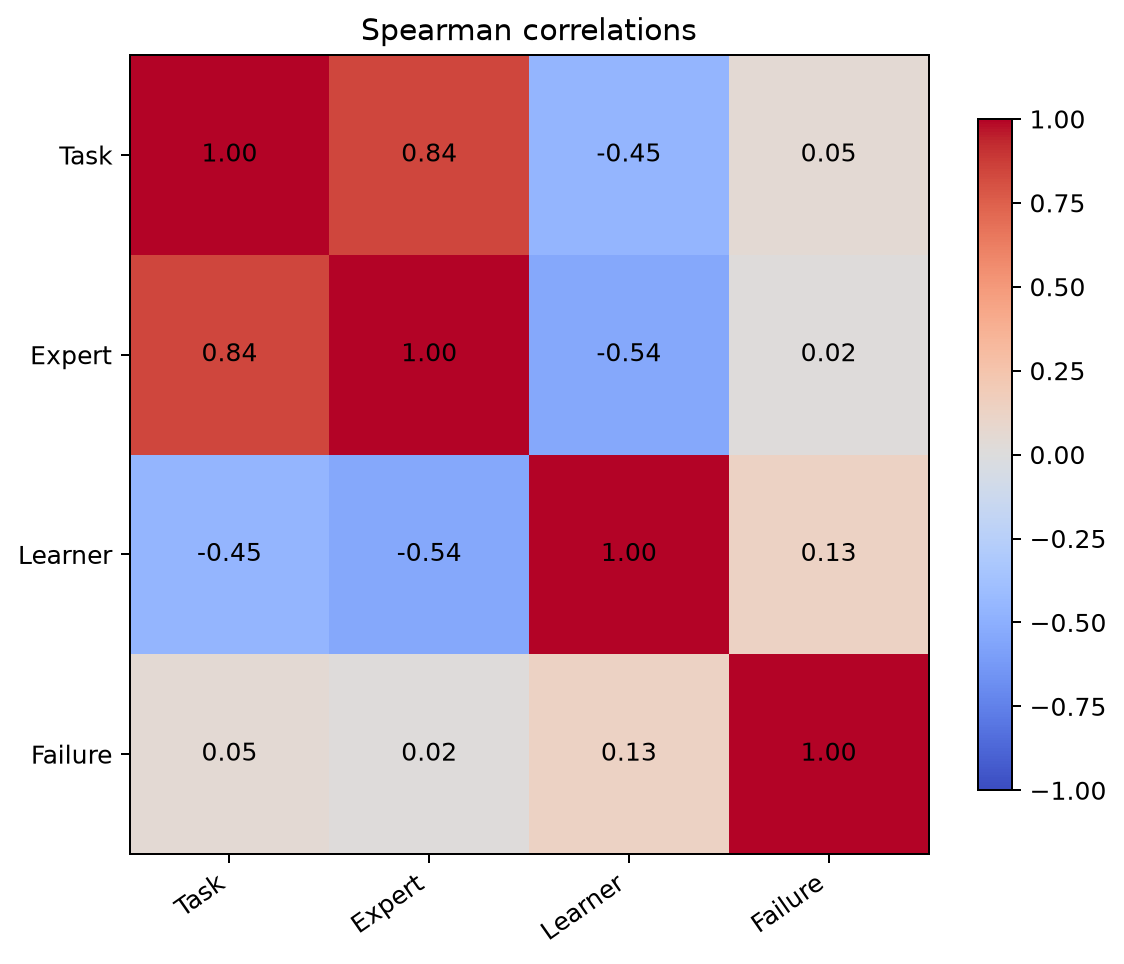
\includegraphics[width=.58\linewidth]{figures/pnp_difficulty_correlation.png}
  \caption{Spearman correlations among Task, Expert, and Learner scores and
  binary out-of-fold rollout failure. The weak score--failure correlations
  complement the AUROC analysis; Learner difficulty disagrees with geometry
  and expert effort.}
  \label{fig:pnp-corr}
\end{figure}

We next reconstruct each demonstrated task and run its out-of-fold policy.
The policies solve 198/240 tasks. Failure AUROC is $0.540$ for Task
($95\%$ bootstrap CI $[0.441,0.647]$), $0.512$ for Expert
($[0.423,0.607]$), and $0.598$ for Learner ($[0.494,0.692]$). Learner has the
largest point estimate, but every interval includes 0.5 and paired-difference
intervals include zero; this does not establish a statistically reliable
winner. Intervals use 1,000 stratified trajectory-level bootstrap resamples.

The Easy/Medium/Hard outcomes also resist a simple interpretation. Task-score
failure rates are 17.5\%, 13.7\%, and 21.3\%; Expert-score rates are 16.2\%,
21.3\%, and 15.0\%; Learner-score rates are 13.7\%, 16.2\%, and 22.5\%.
Only the learner ordering exhibits the intended monotonic increase, and even
there the sample is modest. Grasp and release have the largest expert-phase
prediction errors, while learner-error outliers are unevenly distributed
across OOF folds. A continuous association therefore need not create clean
behavioral regimes after a three-way split.

\subsection{Controlled curriculum learning}
Table~\ref{tab:m7} reports the predefined final checkpoint and normalized
learning-curve AUC. ``Hard'' denotes the 34 hardest of the 100 frozen
development tasks under the Task score using frozen training normalization.
Reverse Learner has the highest observed final and hard-case success, but only
three seeds are available and variance is large.
Its AUC is effectively tied with Uniform, so higher final success should not be
interpreted as clearly faster convergence. Figure~\ref{fig:pnp-curves} shows
the seed-averaged trajectories.

Seed-level outcomes reveal why averages require care. Uniform obtains 80\%,
47\%, and 100\% development success; Task obtains 24\%, 62\%, and 86\%; Expert
obtains 61\%, 61\%, and 37\%; Learner obtains 88\%, 41\%, and 65\%; and Reverse
Learner obtains 84\%, 72\%, and 98\%. Initial weights are matched across
methods within a seed but intentionally differ across seeds. The high spread
is therefore part of the training outcome rather than evaluation-task noise.
Offline validation losses cluster narrowly between 0.00591 and 0.00661 and do
not reproduce the rollout ordering, further motivating closed-loop evaluation.

\begin{table}[t]
\centering
\caption{Pick-and-place development results on 100 frozen tasks, mean $\pm$
sample SD over three seeds. Hard success uses the 34 Task-Hard tasks. Bold
marks only the largest observed mean, not statistical significance.}
\label{tab:m7}
\small
\begin{tabular}{lccc}
\toprule
Method & Final success & Learning AUC & Hard success \\
\midrule
Uniform & $75.7\!\pm\!26.8$ & $0.784\!\pm\!0.054$ & $66.7\!\pm\!32.4$ \\
Task & $57.3\!\pm\!31.3$ & $0.588\!\pm\!0.203$ & $51.0\!\pm\!35.1$ \\
Expert & $53.0\!\pm\!13.9$ & $0.611\!\pm\!0.099$ & $52.0\!\pm\!17.2$ \\
Learner & $64.7\!\pm\!23.5$ & $0.604\!\pm\!0.136$ & $62.7\!\pm\!23.8$ \\
Reverse Learner & $\mathbf{84.7\!\pm\!13.0}$ & $0.787\!\pm\!0.003$ & $\mathbf{91.2\!\pm\!7.8}$ \\
\bottomrule
\end{tabular}
\end{table}

Difficulty-stratified Fresh-ID performance provides a complementary view.
Uniform achieves 74.1\%, 72.6\%, and 61.1\% on Task-defined Easy, Medium, and
Hard groups. Reverse Learner achieves 82.6\%, 78.6\%, and 83.3\%. Groups are
fixed using training-set task-score normalization before observing outcomes.
They represent task-defined strata, not calibrated probabilities of failure.
Likewise, paired comparisons over 200 tasks describe task-level differences
but do not replace independent training seeds.

\begin{figure}[t]
  \centering
  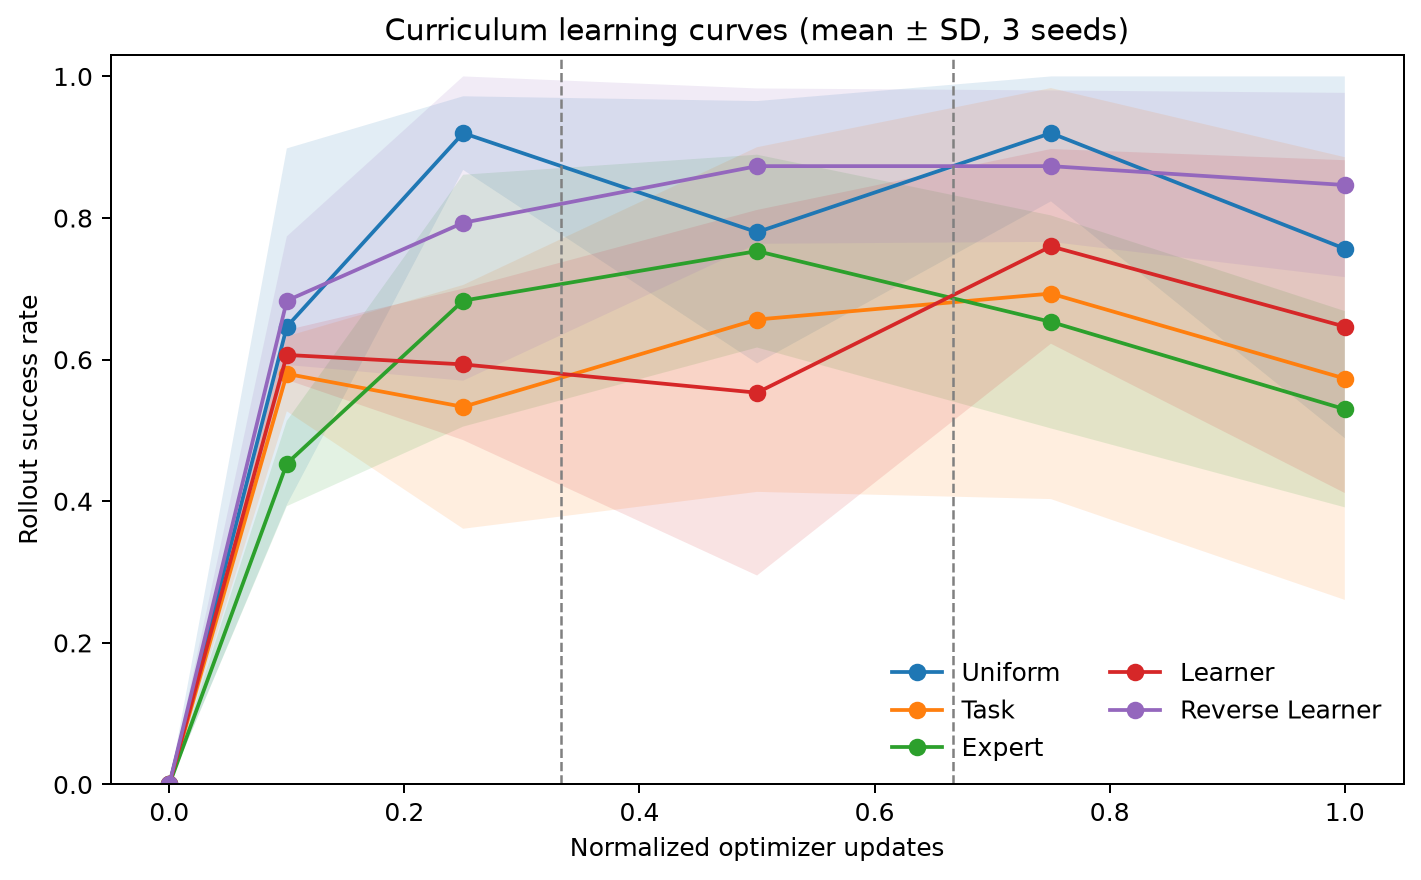
\includegraphics[width=.72\linewidth]{figures/pnp_learning_curves.png}
  \caption{Pick-and-place closed-loop learning curves (mean $\pm$ sample SD)
  on 100 frozen development tasks. Evaluations occur at initialization and at
  10, 25, 50, 75, and 100\% of updates; dashed lines mark stage boundaries.
  AUC integrates success over normalized progress, including update zero.
  Curves do not select the final model.}
  \label{fig:pnp-curves}
\end{figure}

\subsection{Fresh-ID and out-of-distribution evaluation}
\label{sec:final-eval}
Table~\ref{tab:m8} evaluates the final 20,600-update checkpoint on 200 frozen
Fresh-ID tasks, 100 Precision-OOD tasks with unchanged spatial ranges but
radius $[0.030,0.044]$~m, and 100 Spatial-OOD tasks with cube $x$ shifted to
$[0.390,0.415]$~m while other ranges remain standard.
Reverse Learner has the highest mean on all three splits, followed by Uniform
on Fresh-ID. Nevertheless, several OOD means exceed their ID counterpart, so
OOD should not be equated automatically with greater empirical difficulty.
Precision-OOD also tightens a criterion that the policy does not directly
observe, because target radius is absent from the 10D state.

\begin{table}[t]
\centering
\caption{Pick-and-place final success (\%), mean $\pm$ sample SD across three
training seeds. Bold marks only the largest observed mean.}
\label{tab:m8}
\small
\begin{tabular}{lccc}
\toprule
Method & Fresh-ID & Precision-OOD & Spatial-OOD \\
\midrule
Uniform & $69.3\!\pm\!30.4$ & $66.3\!\pm\!30.7$ & $80.7\!\pm\!12.6$ \\
Task & $59.8\!\pm\!29.8$ & $59.3\!\pm\!29.9$ & $39.7\!\pm\!18.6$ \\
Expert & $56.5\!\pm\!10.4$ & $50.3\!\pm\!18.9$ & $61.0\!\pm\!3.0$ \\
Learner & $64.8\!\pm\!21.2$ & $59.3\!\pm\!26.8$ & $46.0\!\pm\!11.1$ \\
Reverse Learner & $\mathbf{81.5\!\pm\!15.7}$ & $\mathbf{79.7\!\pm\!17.0}$ & $\mathbf{81.3\!\pm\!9.3}$ \\
\bottomrule
\end{tabular}
\end{table}

\subsection{Ranking robustness and cross-task observation}
We corrupt the Learner ranking used by Reverse Learner while preserving the
staged schedule and matched seeds. At 25\% or 50\%, that fraction of 240 rank
positions is selected once and the IDs at those positions are permuted; at
100\%, all IDs are randomly permuted. Mean final development success is 84.7\%
at 0\%, 84.3\% at 25\%, 63.7\% at 50\%, and 69.0\% for the random ranking.
Each level has one frozen ranking realization and three training seeds, so the
non-monotonic result is exploratory.

\begin{figure}[!htbp]
  \centering
  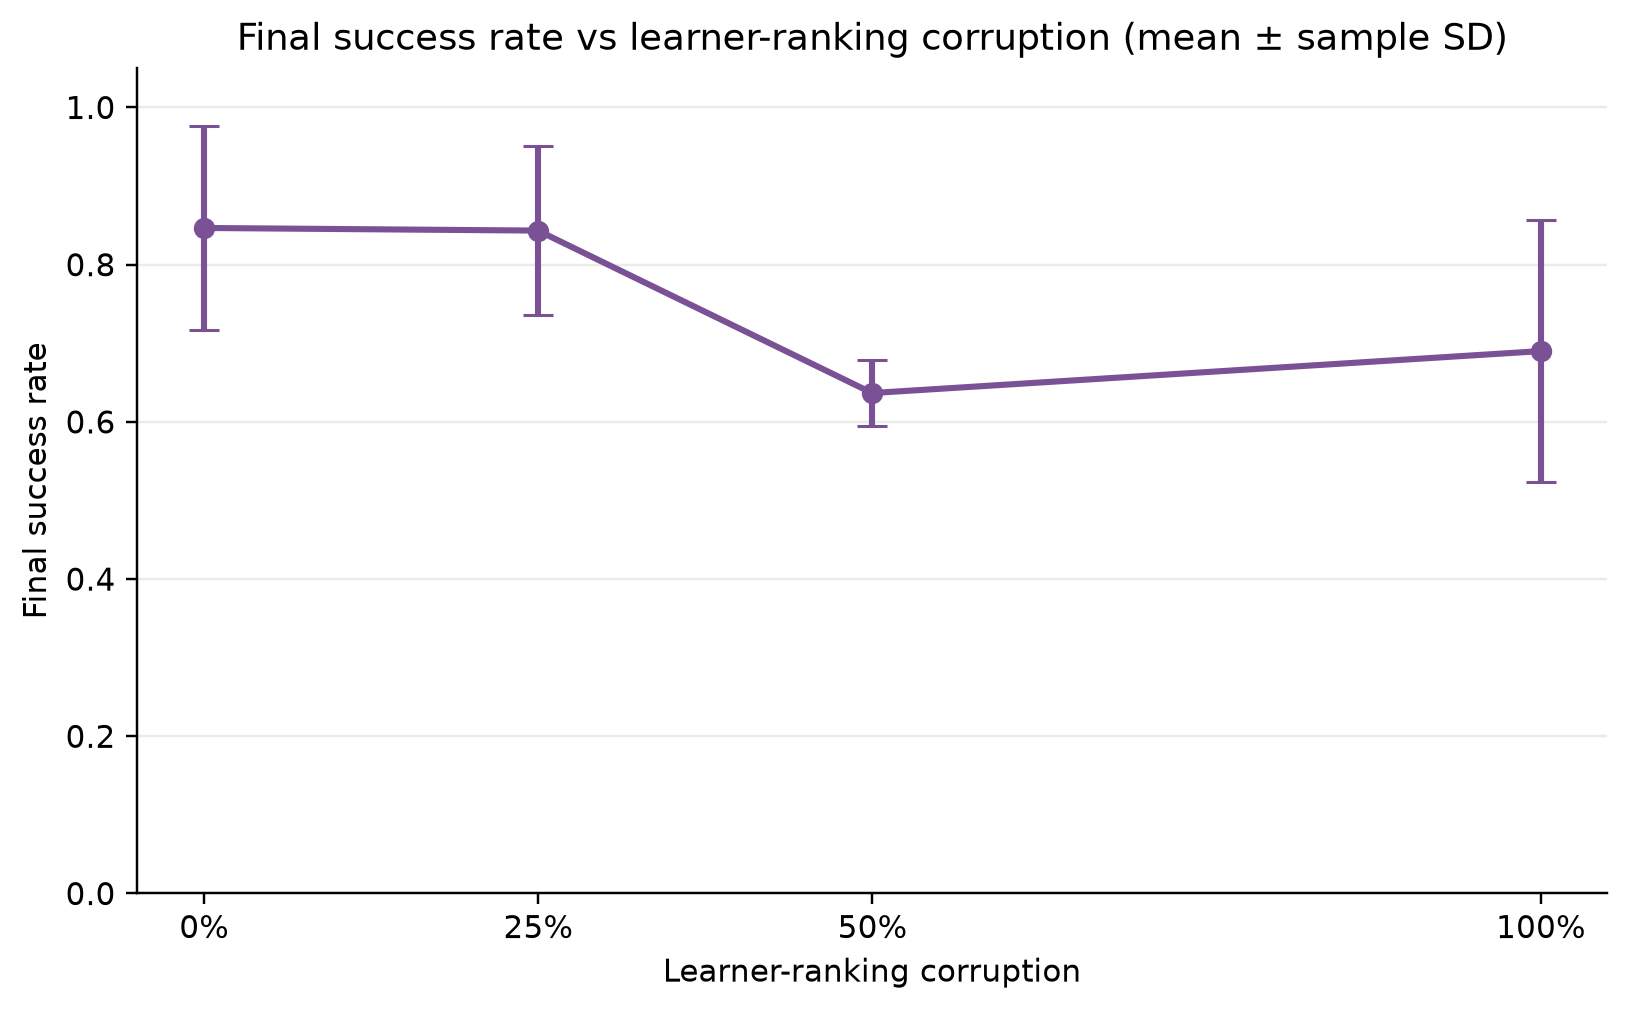
\includegraphics[width=.58\linewidth]{figures/pnp_ranking_robustness.png}
  \caption{Reverse Learner development success under one pre-frozen ranking
  realization per level; 100\% is a fully random permutation. Error bars are
  sample SD across three matched training seeds.}
  \label{fig:robustness}
\end{figure}

The 25\% condition is essentially unchanged, while 50\% corruption degrades
final and hard-group success. A fully random ranking partially recovers. This
may reflect interactions among stage composition, optimization, and the finite
trajectory set rather than one scalar notion of ranking quality. A reliable
response curve would require multiple independent corruptions per level and
more training seeds.

A second task provides an exploratory near-floor comparison. On stacking,
Uniform obtains
$8.33\!\pm\!5.75$\% Fresh-ID success, while Reverse Learner obtains
$2.50\!\pm\!2.00$\%; no curriculum exceeds Uniform. Appendix~\ref{app:stacking}
gives the full experiment. Low success, different representations,
precision-phase emphasis, and different physical criteria prevent treating
this as a decisive reversal or attributing it to task identity alone.
